%%This is a very basic article template.
%%There is just one section and two subsections.
\documentclass{article}
\usepackage[ansinew]{inputenc}
\usepackage{listings}
\usepackage{caption}
\usepackage{color}
\usepackage{xcolor}
\usepackage{cite}
\usepackage{amsmath}
\usepackage{mathtools}
 \definecolor{middlegray}{rgb}{0.5,0.5,0.5}
 \definecolor{lightgray}{rgb}{0.8,0.8,0.8}
 \definecolor{orange}{rgb}{0.8,0.3,0.3}
 \definecolor{yac}{rgb}{0.6,0.6,0.1}

\renewcommand{\lstlistingname}{Codebeispiel}

 \lstset{
   basicstyle=\scriptsize\ttfamily,
   keywordstyle=\bfseries\ttfamily\color{orange},
   stringstyle=\color{green}\ttfamily,
   commentstyle=\color{middlegray}\ttfamily,
   emph={square}, 
   emphstyle=\color{blue}\texttt,
   emph={[2]root,base},
   emphstyle={[2]\color{yac}\texttt},
   showstringspaces=false,
   flexiblecolumns=false,
   tabsize=2,
   numbers=left,
   numberstyle=\tiny,
   numberblanklines=false,
   stepnumber=1,
   numbersep=10pt,
   xleftmargin=15pt,
   captionpos=b,
   sensitive=true
 }

\lstdefinestyle{customc}{  
  belowcaptionskip=1\baselineskip,
  breaklines=true,
  frame=L,
  xleftmargin=\parindent,
  language=C,
  otherkeywords={uint32_t,uint8_t,uint64_t,uint16_t,triplet},
  showstringspaces=false,
  basicstyle=\footnotesize\ttfamily,
  keywordstyle=\bfseries\color{green!40!black},
  commentstyle=\itshape\color{purple!40!black},
  identifierstyle=\color{blue},
  stringstyle=\color{orange},
  sensitive=true
}

\lstset{style=customc, language=C}

\setlength{\parindent}{0pt}
%%=================================


\title{Implementierung der FEAL-Differentrial-Cryptanalysis Attacke nach Murphy}
\author{
	Lukas Becker\\
	\and
	Juri Golanov\\
}


\begin{document}

\maketitle{}
\newpage
\renewcommand{\contentsname}{Inhaltsverzeichnis}
\tableofcontents

%%Kurze Einleitung. Was ist die Problemstellung?
%%Was wird in diesem Paper erl�utert
\section{Einleitung}
Seit jehher herrscht in der Kryptographie ein Rennen zwischen Forschern, die
neue Verfahren entwickeln und Leuten, welche die Schwachstellen in den Verfahren
suchen, um diese f�r ihre Zwecke auszunutzen. Bei der Suche nach \emph{dem}
sicheren Krypto-Verfahren helfen Paper, wie das von Sean
Murphy\cite{attackePaper}. Sie zeigen den Forschern die Schwachstellen ihrer
Algorithmen auf und wie diese in einer Attacke ausgenutzt werden. Durch diese
Erkenntnisse k�nnen dann alte Verfahren verbessert oder neue entwickelt werden,
um die jetzt bekannten Schw�chen zu beseitigen.\par\bigskip

In der folgenden Ausarbeitung werden wir uns der Implementierung der 
\emph{Krypto-Attacke auf den FEAL Algorithmus mit 20 Plaintextbl�cken oder weniger}\cite{attackePaper} von
Sean Murphy befassen. 

\subsection{Aufbau}
Zun�chst werden wir das FEAL Krypto-Verfahren an sich beleuchten. Dazu geh�ren
einmal der Aufbau der Logik, sowie die verwendeten Algorithmen und Funktionen.
\par
Im n�chsten Schritt wird auf die von Sean Murphy entwickelte Attacke
eingegangen. Hier wird vorallem aufgezeigt welche Schw�chen Murphy in dem
Verfahren entdeckt hat und wie er diese ausnutzt.
\par
Nach der Theorie folgt dann die Implementierung der Attacke. Dieses Kapitel
beschreibt �berwiegend den Projektverlauf vom ersten Auseinandersetzen mit dem
Paper bis hin zum fertigen Programm.
\par
Im Anschluss wird ein Fallbeispiel einer Attacke durchgespielt, um zu
veranschaulichen wie das Programm, also die Attacke, vorgeht, um verschl�sselte
Texte ohne Wissen des Schl�ssels zu entschl�sseln.
\par
Danach wird auf Probleme eingangen, denen wir beim Bew�ltigen des Problems
begegnet sind, sowie der resultierende L�sungsweg.
\par
Abschlie�end folgt eine kurze Konklusion zu dem fertigen Projekt.



%%Erkl�rung wie der FEAL Algorithmus funktioniert. (Bezug auf Paper!)
\section{FEAL}
FEAL-N steht f�r \emph{Fast Data Encipherment Algorithm} und ist eine
Blockchiffre, welches auf dem Feistel-Algorithmus basiert, zudem ist es ein symmetrisches 
Kryptoverfahren. FEAL wurde im Jahre 1987 von dem Entwicklerteam Akihiro Shimizu
und Shoji Miyaguchi des japanischen Telefonkonzerns \emph{Nippon Telegraph and
Telephone} (NTT) ver�ffentlicht \cite{fealPaper}. Das Ziel der Entwicklung war
es einen schnellen Verschl�sselungsalgorithmus zu schaffen, der sich effizient in
Software zu implementieren lie�. Es sollte eine Alternative zu dem symmetrischen
Verschl�sselungsalgorithmus \emph{Data Encryption Standard} (DES) darstellen,
welches von der US-Regierung entwickelt wurde und sich damals nur leicht in spezielle
Hardware implementieren lie�. \par\bigskip Das N in FEAL-N repr�sentiert die
Anzahl der Runden der Feistel-Blockchiffren-Operationen auf 64-Bit gro�en
Bl�cke bestimmt durch 64-Bit gro�e Schl�ssel. Diese Ausarbeitung befasst sich
ausschlie�lich mit der Version FEAL-4.\par\bigskip Die folgenden Punkte zeigen
auf, wann, wo und von wem die verschiedenen Versionen von FEAL erfolgreich
gebrochen werden konnten:\par

\begin{itemize}
\item \textbf{FEAL-4} noch im gleichen Jahr 1988 auf der Eurocrypt '88 von B.
den Boer
\item \textbf{FEAL-4} im Jahr 1990 von Sean Murphy mit differentieller
Kryptoanalyse unter Verwendung 20 gew�hlter Plaintextbl�cke (Thema dieser Ausarbeitung)
\item \textbf{FEAL-8} im Jahr 1989 von Biham und Shamir auf der Konferenz
SECURICOM '89
\item \textbf{FEAL-N} mit einer variablen Anzahl an Runden und \textbf{FEAL-NX}
mit 128 Bit langen Schl�ssel statt 64 Bit auf der SECURICOM '91 wieder von Biham und Shamir
\end{itemize}

\par
FEAL hat sich aufgrund zahlreicher Sicherheitsm�ngel nicht durchgesetzt und
sollte bei sicherheitskritischen Anwendungen nicht mehr verwendet werden. Es dient 
heutzutage vor allem zum Testen neuer kryptoanalytischen Angriffsmethoden.
\par\bigskip
------------------------ABSATZ

\subsection{Kurzer Exkurs: Feistel}
Eine Feistel-Chiffre besteht aus einer bestimmten Anzahl an Runden, wobei
jeweils aus dem Schl�ssel ein Rundenschl�ssel gebildet wird. Die untere
Abbildung zeigt die typische Vorgehensweise des Feistel-Algorithmus.
\par

\begin{figure}[h]
\begin{center}
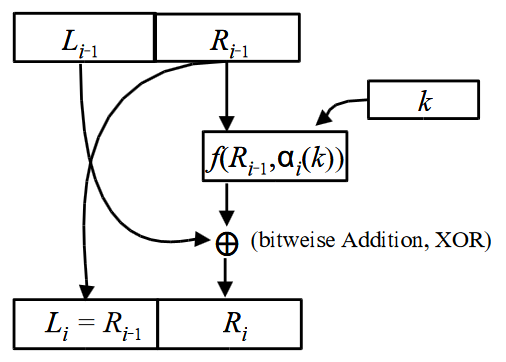
\includegraphics[width=8cm]{tmp/Bilder/feistel.PNG}
\caption{Feistelchiffre}
\end{center}
\end{figure}

\par
Vor jeder Runde wird der Text in eine linke (\textit{L}) und eine rechte H�lfte
(\textit{R}) eingeteilt. Dann wird auf die rechte H�lfte eine Funktion
\textit{f} angewandt, die Teile des Schl�ssels bzw. des sogenannten
Rundenschl�ssels \textit{k} zus�tzlich als Parameter mitbekommt. Das Ergebnis
wird mit XOR ($\oplus$) mit der linken Texth�lfte verkn�pft. Das Ergebnis ist
dann die rechte Texth�lfte f�r die n�chste Runde. Die alte rechte Texth�lfte
wird die neue linke. Der Parameter \textit{i} steht f�r die Anzahl der Runden.
Wie der Feistel-Chiffre im FEAL-4 angewandt wird, wird im folgendem Abschnitt behandelt.
\par\bigskip
\subsection{Funktionsweise}
In diesem Abschnitt wird detailliert auf die Vorgehensweise des Algorithmus
eingegangen, wie das Verschl�sselungsverfahren FEAL-4 funktioniert. Es werden
Funktionen vorgestellt und erkl�rt zu welchem Zweck diese dienen. Zum groben
Ablauf wird zun�chst einmal aufgezeigt wie aus dem 64-Bit Schl�ssel die Subkeys
generiert werden, danach wie Klartexte verschl�sselt und dementsprechend wieder
entschl�sselt werden. Dieser Abschnitt richtet sich nach dem Paper von Sean
Murphy \cite{attackePaper}.
\par
Zu aller erst wird die S-Box-Funktion vorgestellt, diese ist der
Grundbestandteil der wichtigsten Funktionen im FEAL. Diese sieht folgenderma�en aus:
\begin{align*}
S_i(x,y)=Rot_2((x+y+i) Mod 256)
\end{align*}
Der Parameter $i$ ist entweder 0 oder 1, $x$ und $y$ sind 8-Bit gro�e bin�re
Zahlen im Bereich von 0 bis 255. $Rot_2$ entspricht einer Rotation nach links um zwei Bit. 
Das Ergebnis/Output der S-Box-Funktion entspricht einer 8-Bit gro�en bin�ren Zahl.
\par\bigskip
\subsubsection{Generierung der Subkeys}
Aus dem 64-Bit Key sollen zw�lf 16-Bit Subkeys entstehen, welche anschlie�end
verwendet werden, um die Klartexte zu Verschl�sseln. Damit man von den Subkeys
aus nicht so einfach auf den urspr�nglichen Schl�ssel schlie�en kann, werden die
Bits des Keys in mehreren Stufen systematisch durcheinandergebracht.
\par
Als erstes wird dazu der Key in zwei H�lften aufgeteilt. Dazu werden die 32-Bit
langen Hilfsvariablen $B$ ben�tigt, diese erstecken sich von $B_{-2}$ bis $B_6$.
Dabei wird der linke Teil des Keys ($K_L$) der Variable $B_{-1}$ der rechte Teil
des ($K_R$) Keys der Variable $B_0$ zugeordnet, die Variable $B_{-2}$ ist auf
null gesetzt.
\begin{align*}
B_{-2}=0; \qquad B_{-1}=K_L; \qquad B_0=K_R
\end{align*}
\par
Die linken und rechten H�lften von $B_1$ bis $B_6$ sind die gesuchten Subkeys,
sie werden mithilfe der oben genannten Hilfsvariablen und der $f_k$-Funktion
folgenderma�en berechnet.
\begin{align*}
B_i=f_k (B_{i-2},B_{i-1}\oplusB_{i-3})
\end{align*}
In der oberen Gleichung wird die $f_k$-Funktion verwendet, diese ist f�r das
\textit{Verw�rfeln} der Bits zust�ndig. In nachstehender Abbildung wird die
$f_k$-Funktion veranschaulicht, weiterhin sind die dazugeh�rigen Gleichungen
aufgelistet.
\begin{align*}
c= f_k (a,b)
\end{align*}

\par
\begin{figure}[h]
\begin{center}
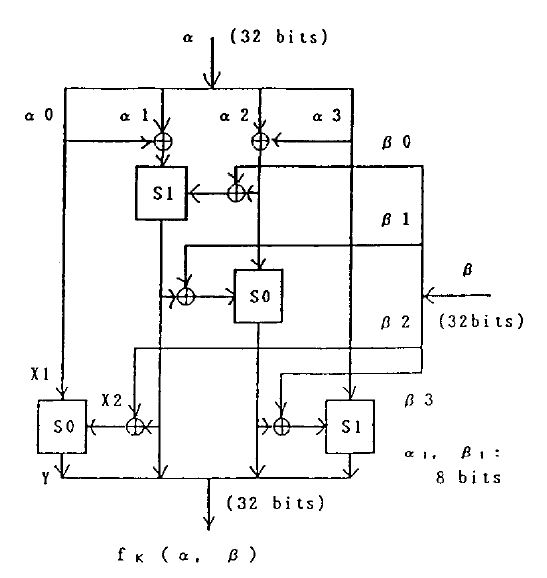
\includegraphics[width=8cm]{tmp/Bilder/fk_funktion.PNG}
\caption{\textit{fk}-Funktion}
\end{center}
\end{figure}
---------------------Bild an falscher Stelle

\begin{gather*}
d_1= a_0 \oplus a_1\\
d_2= a_2 \oplus a_3\\
c_1= S_1 (d_1,d_2 \oplus b_0)\\
c_2= S_0 (d_2,c_1 \oplus b_1)\\
c_0= S_0 (a_0,c_1 \oplus b_2)\\
c_3= S_1 (a_3,c_2 \oplus b_3)\\
\end{gather*}
\par
Die 32-Bit gro�en Bitbl�cke $a$ und $b$ stellen den Input dar. Diese werden
anschlie�end in vier 8-Bit gro�e Teilbl�cke $a_i$ und $b_i$ unterteilt ($i$ = 0,
�, 3), welche mithilfe der S-Box-Funktion und der XOR-Operation miteinander
\textit{vermischt} werden. Daraus resultieren sich die Variablen $c_i$, welche
zusammengesetzt das 32-Bit lange Ergebnis der Funktion liefert.
\par
Zu guter Letzt werden die Hilfsvariablen $B_1$ bis $B_6$ aufgeteilt und als die
endg�ltigen Subkeys verwendet. Aus den sechs 32-Bit langen Hilfsvariablen
entstehen nun die zw�lf 16-Bit langen Subkeys $K_0$ bis $K_{11}$.
\begin{align*}
K_{2(i-1)}= B_i^{L}; \qquad K_{2i-1}= B_i^{R} 
\end{align*}
\par
Aus oberer Gleichung resultiert folgendes Ergebnis in Worten: die sechs gerade
nummerierten Subkeys $K_0$ bis $K_{10}$ bilden die linken H�lften von $B$ und
die sechs ungerade nummerierten Subkeys $K_1$ bis $K_{11}$ bilden die rechten
H�lften von $B$.
\par
Im Folgendem wird der oben aufgezeigte Vorgang vereinfacht dargestellt. Dazu
dient die untere Abbildung, die die Generierung der Subkeys visuell darstellt
und verst�ndlicher macht. Zu erw�hnen ist, dass in folgender Abbildung zwei
Schritte ausgelassen wurden. Die Erstellung der Subkeys $K_8$ bis $K_{11}$ muss
man sich dazu denken.
\par

\begin{figure}[h]
\begin{center}
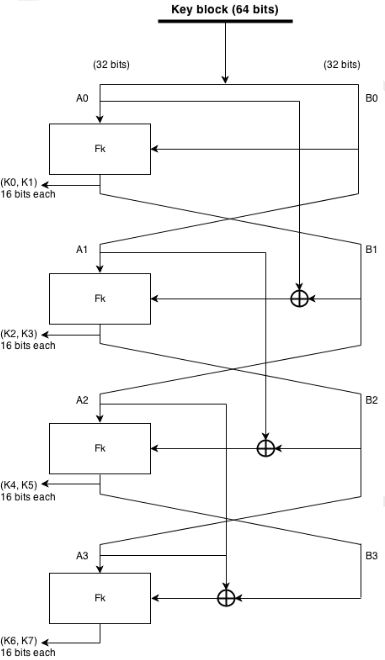
\includegraphics[width=8cm]{tmp/Bilder/subkeys.PNG}
\caption{Erstellung der Subkeys vereinfacht}
\end{center}
\end{figure}
\par
-----------------Bild an falscher Stelle
\par\bigskip
\subsubsection{Verschl�sselung der Klartexte}
Das Verschl�sseln eines 64-Bit gro�en Klartextblockes $P$ erfolgt erneut durch
Aufteilung des Blockes in eine linke ($P_L$) und eine rechte ($P_R$) H�lfte.
Diese werden mit den Subkeys per XOR-Operation miteinander verkn�pft und als
Initialzustand f�r den Feistel-Chiffre genommen. Dazu werden die Variablen $L_0$
und $R_0$ verwendet und werden wie folgt berechnet.
\begin{gather*}
L_0= P_L \oplus (K_4,K_5)\\
R_0= P_L \oplus P_R \oplus (K_4,K_5 ) \oplus (K_6,K_7 )
\end{gather*}
\par
Von hier aus werden nun die vier Runden des Feistel-Algorithmus angewendet.
Daf�r wird die $f$-Funktion und die ersten vier Subkeys $K_0$ bis $K_3$ benutzt.
Die $f$-Funktion ist der $f_k$-Funktion von der Form sehr �hnlich und wird in
der unteren Abbildung veranschaulicht, die entsprechenden Gleichungen sind ebenfalls
aufgef�hrt.
\begin{align*}
c=f(a,b)
\end{align*}
\par

\begin{figure}[h]
\begin{center}
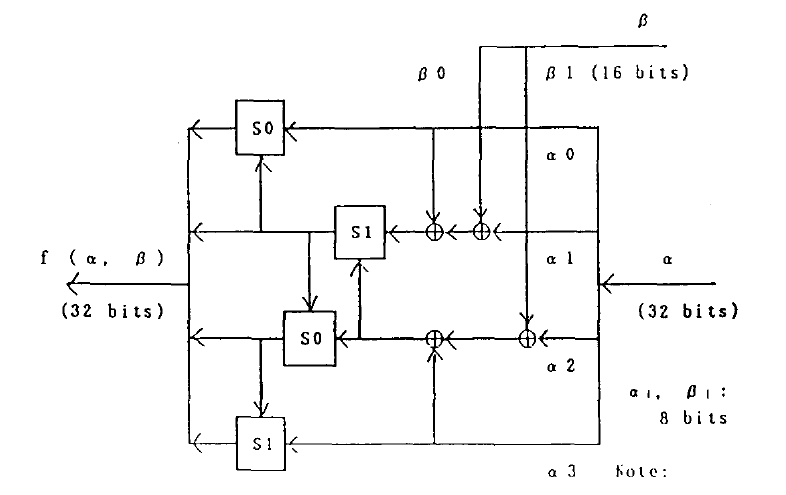
\includegraphics[width=8cm]{tmp/Bilder/f_funktion.PNG}
\caption{\textit{f}-Funktion}
\end{center}
\end{figure}
-----------------Bild an falscher Stelle
\begin{gather*}
d_1= a_0 \oplusa_1\oplus b_1\\
d_2= a_2 \oplusa_3\oplus b_2\\
c_1= S_1 (d_1,d_2)\\
c_2= S_0 (d_2,c_1)\\
c_0= S_0 (a_0,c_1)\\
c_3= S_1 (a_3,c_2)\\
\end{gather*}
\par
Die Gleichung f�r den Durchlauf der vier Feistel-Runden sieht wie folgt aus, f�r
$i$=0,1,2,3 :
\begin{gather*}
L_i= R_{i-1}\\
R_i= L_{i-1} \oplus f(R_{i-1},K_{i-1})
\end{gather*}
\par
Die daraus resultierenden Ergebnisse des Feistel-Algorithmus $L_4$ und $R_4$
werden abschlie�end mit den letzten vier Subkeys $K_8$ bis $K_{11}$ per XOR
miteinander verkn�pft und den Variablen $C_L$ und $C_R$ zugewiesen.
\par
\begin{gather*}
C_L= R_4 \oplus (K_8,K_9)\\
C_R= R_4 \oplus L_4 \oplus (K_{10},K_{11})
\end{gather*}
\par
Daraus ergibt sich zu guter Letzt der verschl�sselte Ciphertextblock $C$ mit
\begin{align*}
C=(C_L,C_R).
\end{align*}
\par
Auf die gleiche Weise k�nnen wir, wenn wir den Schl�ssel kennen, jede
verschl�sselte Nachricht dekodieren, indem die oben beschriebene Vorgehensweise
einfach in umgekehrter Reihenfolge angewendet wird. Die unteren Abbildungen
vereinfachen die oben im Detail beschriebene Vorgehensweise des Verschl�sselns
und veranschaulichen als Gegenst�ck den Vorgang des Entschl�sselns.
\par
\begin{figure}[h]
\begin{center}
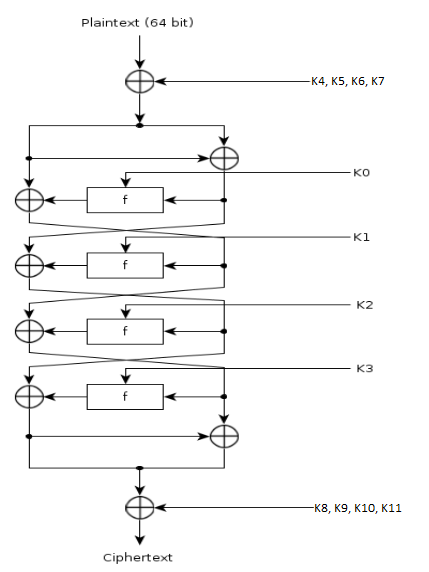
\includegraphics[width=10cm]{tmp/Bilder/encode.PNG}
\caption{Encode vereinfacht}
\end{center}
\end{figure}
-----------------Bild an falscher Stelle
\par
\begin{figure}[h]
\begin{center}
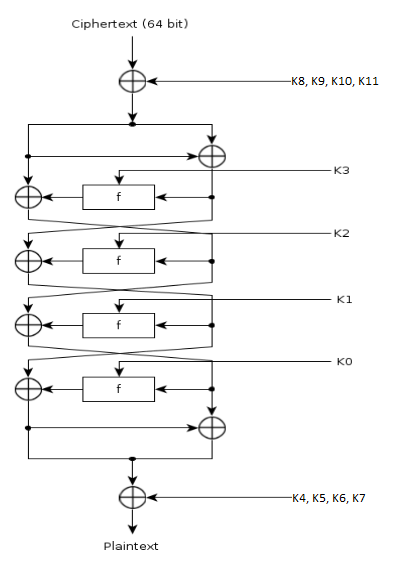
\includegraphics[width=10cm]{tmp/Bilder/decode.PNG}
\caption{Decode vereinfacht}
\end{center}
\end{figure}
-----------------Bild an falscher Stelle
\par

%%Erkl�rung wie die Attacke funktionieren soll. (Bezug auf Murphy!)
\section{Attacke nach Murphy}

%%Erkl�rung wie wir FEAL & Attacke implementiert haben.
\section{Implementierung}
Im folgenden Abschnitt werden wir sowohl auf die Implementierung des
\emph{FEAL-4} Verfahren, als auch auf die der Attacke eingehen. Als
Programmiersprache wurde C gew�hlt, da ein kompiliertes Programm eine h�here Performanz
besitzt als zum Beispiel ein Java Programm, welches �ber einen Interpreter
l�uft.\par
Die Software wurde in drei Teilkomponenten unterteilt. Einmal die
FEAL Komponente, welche alle Funktionen besitzt, um die Funktionalit�t des
FEAL Verfahrens bereitzustellen. Die n�chste Komponente widmet sich ganz
der Attacke, welche von Murphy beschrieben wurde. Abschlie�end gibt es noch
eine Verifizierer Komponente. Diese dient zur Verfikation aller Funktionen,
die in den beiden anderen Komponenten erstellt wurden.\par
Bevor wir jedoch die einzelnen Komponenten uns im Detail betrachten, werden erst
einige Grundkonventionen festgelegt. Diese dienen zur Vereinheitlichung und zum 
besseren Nachvollziehen des Codes im Bezug auf das vorgegebene 
Paper\cite{attackePaper}.\par\bigskip

\subsection{Konventionen}
Da Murphy in seinem Paper die meisten Funktionalit�ten sowohl des FEAL, als
auch des Attacke-Algorithmus als mathematische Funktionen dargestellt hat, ist
der �bergang von der Theorie in die Implementierung verh�ltnisweise einfach. Um
den Bezug auf die mathematischen Funktionen nicht zu verlieren, wurde die
Mehrzahl der Variablennamen eins zu eins �bertragen. Ausnahmen waren zum
Beispiel die Bytevariablen eines gesplitteten Doppelwortes. Nehmen wir an eine
32-Bit Zahl h�tte den Variablennamen \textit{a}. So haben in dem Paper die 4
Teilbytes von \textit{a} einen zus�tzlichen fortlaufenden Index, also
\textit{a0, a1, a2, a3}. Unsere Implementierung realisiert eine gesplittete
32-Bit Zahl als Byte-Array der L�nge 4 und beh�lt dabei den Variablennamen
aus dem Paper. Damit �hnelt ein Zugriff auf den entsprechenden Index im Array (z.B.
\textit{a[1]}) dem aus dem Paper (\textit{a1}). Damit sich der Namensbereich des
Arrays und der initialen 32-Bit Zahl nicht �berschneidet, wird der initialen
Zahl ihre Gr��enbezeichnung an den Variablennamen des Papers angehangen. In
unserem Beispiel h�tte die \textit{UInt32} Repr�sentation von \textit{a} also
den Variablennamen \textit{aDWord}.\par
F�r erstellte Funktionen gelten die selben Namenskonventionen. Falls eine
Funktion von Murphy explizit in einer mathematischen Repr�sentierung vorhanden
ist, wird der Name dieser Funktion �bernommen. Beinhaltet der Funktionname einen 
griechischen Buchstaben (z.B. $\theta$), so wird in der Implementierung der
Buchstabe anhand des repr�sentativen Wortes aus lateinischen Buchstaben
ausgeschrieben (z.B. \textit{theta}). Wird eine Funktion nicht explizit im Paper
genannt oder niedergeschrieben, so ist f�r sie ein ad�quater Funktionsname, der
die �blichen Programmierkonventionen einh�lt zu w�hlen.\par\bigskip

\subsection{Implementierung explizit formulierter Funktionen}
Wie bereits erw�hnt werden die meisten Funktionen in dem Paper von Murphy
explizit ausformuliert. Um besser nachvollziehen zu k�nnen, wie der
Implementierungsprozess einer solchen Funktion abl�uft, wird
nun die Implementierung der Funktion \textit{f} aus dem
Paper\cite{attackePaper} durchgef�hrt.\par
Wir betrachten dabei zuerst folgenden Auszug, welcher die Definition von
\textit{f} beinhaltet:\par\bigskip

Now suppose that $a_i,c_i~\epsilon~Z^8_2$ for $i=$ 0,1,2,3, and also that
$b_1,b_2~\epsilon~Z^8_2$, with $b=(b_1,b_2)~\epsilon~Z^{16}_2$ and
$a=(a_0,a_1,a_2,a_3),c~\epsilon~Z^{32}_2$ etc., then we can define
\begin{gather*}
c = f(a,b)
\end{gather*}
as follows: 
\begin{gather*}
d_1 = a_0 \oplus a_1 \oplus b_1\\
d_2 = a_2 \oplus a_3 \oplus b_2\\
c_1 = S_1(d_1,d_2)\\
c_2 = S_0(d_2,c_1)\\
c_0 = S_0(a_0,c_1)\\
c_3 = S_1(a_3,c_2)
\end{gather*}
Anhand dieser Definition l�sst sich auf alle Eigenschaften unserer zu
implementierenden Funktion schlie�en. Wir sehen, das $f$ die Parameter $a$ und
$b$ besitzt, wobei $a$ definiert ist als Konkatenation von 4 Bytes und $b$ als
eine Konkatenation von 2 Bytes. Des Weiteren k�nnen wir erkennen, das
$f(a,b)=c$, wobei $c$ als 32-Bit Zahl definiert ist. Durch diese Informationen
l�sst sich auf folgende Deklaration in C schlie�en:\par\bigskip
\begin{lstlisting}[caption={Deklartation der Funktion $f$ in C}]
 /**
 * Implementierung der f Funktion aus dem Paper
 *
 * c = f(a, b)
 *
 * @param aDWord - a
 * @param b		 - b
 *
 * @result c (32 bit)
 */
uint32_t f(uint32_t aDWord, uint16_t b);
\end{lstlisting}
Wir k�nnen in der Definition erkennen, das $a$ und $b$ nicht im Ganzen, sondern
ihre jeweiligen Bytes verwendet werden. Das hei�t, das bevor wir die Operationen
aus der Definition implementieren, m�ssen wir eine Funktion aufrufen, die uns
$a$ und $b$ in Bytes aufsplittet. Zudem m�ssen am Schluss die 4 Bytes
$c0,c1,c2,c3$ zu dem Doppelwort $c$ zusammengef�gt werden. Dies f�hrt dann zu
folgender Implementierung von $f$:
\begin{lstlisting}[caption={Implementierung der Funktion $f$ in C},
label=lst:fFunktion]
uint32_t f(uint32_t aDWord, uint16_t b)
{
	uint8_t b2 = (uint8_t) b;
	uint8_t b1 = (uint8_t)(b >> 8);
	uint8_t a[4] = {0};
	uint8_t c0, c1, c2, c3, d1, d2;

	// Split a to a0, a1, a2, a3
	splitToBytes(aDWord, a);

	d1 = a[0] ^ a[1] ^ b1;
	d2 = a[2] ^ a[3] ^ b2;
	c1 = S(d1, d2, ONE);
	c2 = S(d2, c1, ZERO);
	c0 = S(a[0], c1, ZERO);
	c3 = S(a[3], c2, ONE);

	return bytesToUint32(c0, c1, c2, c3);
}
\end{lstlisting}
Anhand dieser Vorgehensweise wurden alle weiteren explizit ausformulierten
Funktionen implementiert. Vorallem die Implementierung des FEAL Verfahren wurde
durch diese Vorgehensweise sehr vereinfacht. Interessant ist nun zu betrachten,
wie die Attacke implementiert wurde.\par\bigskip

\subsection{Implementierung der Attacke}
\label{subsection:ImplementierungAttacke}
In \emph{Krypto-Attacke auf den FEAL Algorithmus mit 20 Plaintextbl�cken oder
weniger}\cite{attackePaper} wird die Attacke haupts�chlich anhand von Prosa
geschildert, mit zus�tzlichem Bezug auf vorher aufgestellte Gleichungen. Dabei
handelt es sich um zwei verschiedene Formen von Gleichungen, die
unterschiedliche Arten der Implementierung mit sich ziehen.\par
Die erste Form sind Gleichungen, wo ein $x$ gesucht wird, welches die Gleichung
l�st. Die Vorgehensweise bei der Suche nach $x$ ist dabei h�ufig das Pr�fen von
anderen Gleichungen, welche mit Bestandteilen von $x$ zusammenh�ngen. Wenn diese
Gleichungen alle erf�llt sind, haben wir eine L�sung f�r $x$. Dies f�hrt dazu,
das nicht nur eine, sondern mehrere L�sungen f�r $x$ gefunden werden.\par
Betrachten wir als Beispiel die Implementierung der Gleichungen (3.7) aus dem
Paper\cite{attackePaper}:
\begin{align*}
G(x \oplus a) \oplus G(x \oplus b) = d\\
G(x \oplus a) \oplus G(x \oplus c) = e
\end{align*}
Wir werden uns an dieser Stelle nur die Implementierung betrachten, welche
verdeutlicht, wie L�sungen f�r ein $x$ gefunden werden. Die Theorie zu der
Implementierung finden Sie in (3.6) des Papers\cite{attackePaper}.
\newpage
\begin{lstlisting}[caption={Implementierung zur Suche von $x$ in
(3.7)\cite{attackePaper}}] 
int getSolutionsForXFrom3_7(uint32_t aDWord, uint32_t
bDWord, uint32_t cDWord, uint32_t dDWord, uint32_t eDWord, 
uint32_t ** solutions) {

	int solutionCount = 0;	// Anzahl an Loesungen fuer x
	uint8_t a[4] = {0};
	uint8_t b[4] = {0};
	uint8_t c[4] = {0};
	uint8_t d[4] = {0};
	uint8_t e[4] = {0};

	// Allokiere Plaetze, um die Loesungen fuer x zu speichern.
	// Nehmen wir an, das 100% aller z1, z2 die Gleichung (3.2) erfuellen.
	// Dann allokieren wir 2^17 * 32 = 4194304 bit = 524288 Byte = 512 KB im Heap.
	// Damit sollten alle moeglichen Loesungen fuer x in diesem Array
	// gespeichert werden koennen.

	//2^17 hat nicht funktioniert, also 131072 ausgeschrieben...
	uint32_t *tmpPointer = malloc(131072 * sizeof(uint32_t));	


	// Split a to a0, a1, a2, a3 (analog fuer b, c, d, e)
	splitToBytes(aDWord, a);
	splitToBytes(bDWord, b);
	splitToBytes(cDWord, c);
	splitToBytes(dDWord, d);
	splitToBytes(eDWord, e);

	uint8_t z1 = 0;
	uint8_t z2 = 0;
	// Check fuer jedes z1, z2...
	for(int i = 0; i < 256; ++i)
	{
		z1 = i;
		for(int j = 0; j < 256; ++j)
		{
			z2 = j;
			// Wir checken fuer beide Gleichungen in (3.7) gleichzeitig!!!
			uint8_t alpha1 = S(z1 ^ a[0] ^ a[1], z2 ^ a[2] ^ a[3], ONE);
			uint8_t beta1  = S(z1 ^ b[0] ^ b[1], z2 ^ b[2] ^ b[3], ONE);
			uint8_t gamma1 = S(z1 ^ c[0] ^ c[1], z2 ^ c[2] ^ c[3], ONE);

			if(((alpha1 ^ beta1) != d[1]) || ((alpha1 ^ gamma1) != e[1]))
				continue;

			uint8_t alpha2 = S(alpha1, z2 ^ a[2] ^ a[3], ZERO);
			uint8_t beta2  = S(beta1, z2 ^ b[2] ^ b[3], ZERO);
			uint8_t gamma2 = S(gamma1, z2 ^ c[2] ^ c[3], ZERO);

			if(((alpha2 ^ beta2) != d[2]) || ((alpha2 ^ gamma2) != e[2]))
				continue;

			for(int k = 0; k < 256; ++k)
			{
				uint8_t x0 = k;
				for(int l = 0; l < 256; ++l)
				{
					uint8_t x3 = l;
					uint8_t s0Alpha1 = S(alpha1, x0 ^ a[0], ZERO);
					if((s0Alpha1 ^ S(beta1, x0 ^ b[0], ZERO)) != d[0])
						continue;

					if((s0Alpha1 ^ S(gamma1, x0 ^ c[0], ZERO)) != e[0])
						continue;

					uint8_t s1Alpha2 = S(alpha2, x3 ^ a[3], ONE);
					if((s1Alpha2 ^ S(beta2, x3 ^ b[3], ONE)) != d[3])
						continue;

					if((s1Alpha2 ^ S(gamma2, x3 ^ c[3], ONE)) != e[3])
						continue;

					// Jede Gleichung fuer z1, z2, x0, x3 ist korrekt.
					// Errechne x1, x2 (3.4) und speichere die Loesung fuer x ab.
					uint32_t x = bytesToUint32(x0, z1 ^ x0, z2 ^ x3, x3);
					tmpPointer[solutionCount] = x;
					++solutionCount;
				}
			}
		}
	}
	*solutions = realloc(tmpPointer, solutionCount * sizeof(uint32_t));
	return solutionCount;
}
\end{lstlisting}
Wie ab Zeile 32 zu sehen ist, traversieren wir durch mehrere for-Schleifen,
wobei jede den Wert einer Komponente �ndert, welche mit $x$ zusammenh�ngt. F�r
diese Werte wird dann gepr�ft, ob sie die n�tigen Gleichungen erf�llen (z.B.
Zeile 43). Falls nicht, kann der Wert f�r diese Komponente verworfen werden. Ist
die Gleichung erf�llt, kann weiter verfahren werden. Sollten alle gew�hlten
Komponentenwerte ihre jeweiligen Gleichungen erf�llen, kann daraus eine L�sung
f�r $x$ generiert werden (Zeile 75). Bei derartigen Funktionen werden die
verschiedenen L�sungen f�r $x$ immer in einer Pointerstruktur gespeichert und
die Anzahl der gefunden L�sungen als Return-Wert zur�ck gegeben.\par\bigskip

Die zweite Form von Gleichungen sind sind quasi Assertions. Im Laufe der Attacke
sollen an bestimmten Punkten gepr�ft werden, ob die bisher gesammelten Werte
bestimmte Gleichungen erf�llen. Dies dient in erster Linie der Reduktion
m�glicher L�sungen. Als Beispiel betrachten wir die Assertion der Gleichung
(5.5) aus dem Paper\cite{attackePaper}:\newpage
\begin{lstlisting}[caption={Implementierung der Assertion f�r Gleichung
(5.5)\cite{attackePaper}}]
/**
 * Prueft, ob die Parameter Gleichung 5.5 erfuellen:
 *
 * 	CiL ^ U0 ^ G(PiL ^ V0) ^ G(Di ^ W) = 0		i = 0 		(5.5)
 *
 * @param CiL
 * @param trippel
 * @param PiL
 * @param Di
 *
 * @return 1, wenn erfuellt ; 0, wenn nicht
 */
int doesSatisfy5_5(uint32_t CiL, struct triplet trippel, uint32_t PiL,
 uint32_t Di)
{
	if(( CiL ^ trippel.U0 ^ G(PiL ^ trippel.V0) ^ G(Di ^ trippel.W)) == 0)
		return 1;
	return 0;
}
\end{lstlisting}
Wie zu sehen, handelt sich dabei um eine einfache if-Abfrage, welche die
Gleichung repr�sentiert. In Zeile 13 wird zum ersten mal die neue Datenstruktur
\emph{triplet} genannt. Diese ist ein f�r die Attacke entwickelte Struktur,
welche auf den Gleichungen (5.3)\cite{attackePaper} beruht:\par\bigskip
\begin{lstlisting}[caption={Datenstruktur f�r die Werte aus
(5.3)\cite{attackePaper}}]
/*
 * Struct fuer das tripel, welches in 5.3 vorgestellt wird
 */
struct triplet{
	uint32_t W;
	uint32_t V0;
	uint32_t U0;
};
\end{lstlisting}
Vorteil dieser Datenstruktur ist eine konsistentere Speicherung von
zusammenh�ngenden $W, V^0$ und $U^0$ Werten. Zus�tzlich erleichtert es die
Nachvollziehbarkeit innerhalb des Codes.\par\bigskip\newpage
Ein weiterer wichtiger Teil der Attacke ist die Wahl der Plaintexte. Schwierig
war dabei 64-Bit Pseudo Zufallszahlen zu generieren, denn die C eigene
Zufallszahlenfunktion \emph{rand()} liefert nur Zahlen im Bereich von 0 bis
\emph{RAND\_MAX}, welches mindestens 32767 ist. Um nun eine 64-Bit Pseudo
Zufallszahl zu generieren wurde die \emph{rand()} Funktion vier mal aufgerufen
und die resultierenden Werte durch bit-shift und xor Operationen zu einer 64-Bit
Zahl zusammen gef�gt. Der folgende Ausschnitt ist ein Beispiel f�r eine solche
Generierung:\par\bigskip
\begin{lstlisting}[caption={Generierung einer 64 bit Pseudo Zufallszahl}]
	P[0]   = ((uint64_t)rand() << 48)^ ((uint64_t)rand() << 32) ^
			((uint32_t)rand() << 16) ^ ((uint32_t)rand());
\end{lstlisting}
Das Herzst�ck unserer Attacke ist die \emph{attack()} Funktion. Sie beinhaltet
einen gesamten Durchlauf einer Attacke, vom W�hlen der Plaintexte bis hin zum
Berechnen der Schl�sselkonstanten. Die Attacke wurde bewusst nicht zu fein
aufgesplittet, um den Weg, der in dem Paper\cite{attackePaper} beschrieben ist,
noch nachvollziehen zu k�nnen. Wir werden an dieser Stelle nicht auf die
detaillierte Implementierung der \emph{attack()} Funktion eingehen. In unserem
Fallbeispiel werden wir die komplette Funktion durchlaufen und an wichtigen
Stellen Codeausschnitte liefern, welche in Summe eine ausreichende Erl�uterung
zur Implementierung sein sollten. Doch bevor wir das Fallbeispiel
betrachten, m�ssen wir zun�chst noch auf die dritte Komponente der
Software eingehen, den Verifizierer.\par\bigskip

\subsection{Implementierung des Verifizierers}
\label{subsection:Verifizierer}
Der Verifizierer stellt in unserer Software eine Kontrollinstanz dar. Um
sicher zu stellen, dass jede Funktion, die f�r \emph{FEAL} oder die Attacke
geschrieben wurde korrekt funktioniert, wurde im Verifizierer jeweils eine
Testfunktion hinterlegt. Jede Testfunktion pr�ft, ob die zu pr�fende Funktion
richtig agiert. Es kann auf verschiedene Arten gepr�ft werden.\par Bei den
Funktionen, die einen Wert zur�cklieferen sollen, wird vorher ein erwartetes
Ergebnis gespeichert. Dieses wird dann mit dem Ergebnis, welches die zu pr�fende
Funktion zur�ck gibt verglichen. Nur wenn erwartetes und tats�chliches Ergebnis
gleich sind, gilt die Funktion als verifiziert.\par Betrachten wir uns als
Beispiel die Funktion $f$ aus dem Codebeispiel \ref{lst:fFunktion}. $f$ gibt f�r ein
bekanntes $a$ und $b$ eine 32-Bit Zahl zur�ck. Das hei�t f�r unsere
Testfunktion, das wir ein $a$ und $b$ festlegen, die $f$ Funktion anhand des
Papers\cite{attackePaper} unabh�ngig von der zu testenden Implementierung
ausf�hren und dieses Ergebnis als Erwartung voraussetzen. Dann wird die zu
testende Funktion mit den Parametern $a$ und $b$ aufgerufen und dieses Ergebnis
gespeichert. Sollten nun das erwartete und tats�chliche Ergebnis gleich sein,
gilt $f$ als verifiziert. Codebeispiel \ref{lst:Verifizierungf} zeigt die
Implementierung einer solchen Testfunktion:\par\bigskip
\begin{lstlisting}[caption={Verifizierung der Funktion $f$}, label=lst:Verifizierungf] 
int verifyFunctionF(int withOutput)
{
	uint32_t a = 0x12345678;
	uint16_t b = 0xbcde;
	uint32_t expected = 0x012e78c7;
	uint32_t result = f(a,b);

	if(withOutput)
	{
		printf("Test f mit a = 0x%" PRIx32", b = 0x%"PRIx32 ". Expected: 0x%"PRIx32" Result: 0x%"PRIx32"\n",
				a, b, expected, result);
	}
	if(expected != result)
		return 0;
	return 1;
}
\end{lstlisting}
Andere Funktionen k�nnen mit Hilfe bereits verifizierter Funktionen auf ihre
Korrektheit gepr�ft werden. Nehmen wir als Beispiel die $decode()$ Funktion f�r
das \emph{FEAL}-Verfahren. Wenn die $encode()$ Funktion bereits verifiziert ist,
l�sst sich die Richtigkeit f�r $decode()$ einfach zeigen. Sollte $decode()$
Ciphertextbl�cke, die von $encode()$ verschl�sselt wurden, wieder in die
urspr�nglichen Plaintexte dekodieren k�nnen, so gilt $decode()$ als verifiziert.
Codebeispiel \ref{lst:Verifizierungdecode} zeigt die Implementierung der
Testfunktion f�r $decode()$:\par\bigskip
\begin{lstlisting}[caption={Verifizierung der Funktion $decode()$},
label=lst:Verifizierungdecode]
int verifyFunctionDecode(int withOutput)
{
	// Testschl�ssel
	uint64_t key = 0xFF00FF00FF00FF00;

	// Zuerst werden die 12 16 bit subkeys errechnet
	uint16_t *subkeys = compSubKeys(key);

	// Danach werden 20 Plaintexte nach der Definition aus dem Paper
	// erzeugt.
	uint64_t *P = choosePlainTexts();

	// Allokiere Speicher fuer die Ciphertextbloecke und wende das 
	// FEAL-Verfahren zur Verschluesselung an.
	uint64_t *C = malloc(20 * sizeof(uint64_t));
	for(int i = 0; i < 20; ++i)
	{
		C[i] = encode(P[i], subkeys);
	}

	// Entschluessel die 20 Ciphertextbloecke und
	// vergleiche, ob sie mit den urspruenglichen Plaintextbloecken 
	// uebereinstimmen.
	uint64_t decodedP[20];
	int isEqual = 1;
	for(int i = 0; i < 20; ++i)
	{
		decodedP[i] = decode(C[i], subkeys);
		if(decodedP[i] != P[i])
		{
			isEqual = 0;
		}
		if(withOutput)
		{
			printf("Urspruenglicher Plaintext: 0x%" PRIx64 "\t", P[i]);
			printf("Dekodierter Plaintext: 0x%" PRIx64"\n", decodedP[i]);
		}
	}

	return isEqual;
}
\end{lstlisting}
Auf diese Weise ist Suche nach Fehlern in der sp�teren fertigen Attacke um
einiges leichter, da man bestimmte aufgerufene Funktionen anhand ihrer
Verifizierung ausschlie�en kann.\par\bigskip Alle in diesem Kapitel genannten
Ma�nahmen f�hrten letztendlich zu einem fertigen Programm, welches erfolgreich die
Krypto-Attacke auf das FEAL-Verfahren durchf�hren kann. Im n�chsten Kapitel wird
nun ein Fallbeispiel einer solchen Attacke erl�utert.


%%Ein Beispieldurchlauf der Attacke.
\section{Fallbeispiel}

%%Probleme bei der Bew�ltigung unserer Aufgabe
\section{Schwierigkeiten und Herausforderungen}


%%Ein paar abschlie�ende Worte zu dem Projekt.
\section{Konklusion}
Die Arbeit an diesem Projekt war f�r uns sehr aufschlussreich. Eine praktische
Erfahrung zu dem bereits vorhandenen theoretischen Wissen hat unseren 
Einblick in das Thema Kryptographie noch weiter gesch�rft. Das Einarbeiten und 
Implementieren einer uns vorher noch unbekannten Attacke gab uns sehr viel
Aufschluss �ber die Herangehensweise der Entwicklung einer Attacke gegen ein
Krypto-Verfahren.\par
Zusammenfassend l�sst sich sagen, dass das Projekt ein Erfolg war und wir 
durchweg positive Erfahrungen mitnehmen.\par\bigskip

\bibliographystyle{ieeetr}
\bibliography{bib}{}
\end{document}
